\documentclass[10pt]{beamer}
\usepackage[utf8]{inputenc}
\usepackage[T1]{fontenc}
\usepackage{lmodern}
\usepackage{latexsym}
\usepackage{graphicx}
\usepackage{amsmath}
\usepackage{amsfonts}
\usepackage{amssymb}
\usepackage[]{babel}
\usepackage{ragged2e}\justifying
\usetheme{Cuerna}
%\usecolortheme{brick}
\begin{document}
	\author{\begin{center}
			Jordan Kevin Buwa Mbouobda \\
			{\small{\textit{Supervisor}}}: Zuzana Mas\'arov\'a	\end{center} }
	\title{Constrained triangulations}
	%\subtitle{}
	\logo{
\includegraphics[scale=.20000]{nm}}
	\institute{\begin{center}
			{\centering African Institute for Mathematical Sciences\\ Ghana}
	\end{center}}
	\date{\today}
	\setbeamertemplate{navigation symbols}{}
	%\textcolor{ \small{Under the supervision of}\\Zuzana Masárová}
	%\setbeamercovered{transparent}
	%\setbeamertemplate{navigation symbols}{}
	\begin{frame}[plain]	
		\maketitle
		%\textcolor{ \small{Under the supervision of}\\Zuzana Masárová}
	\end{frame}
	
	\begin{frame}
		%\titlepage
		\frametitle{Outline}
		\begin{itemize}
			\item Introduction
			%\pause 
			\item Motivation
		%	\pause
			\item Definition
		%	\pause
			\item Line sweeping algorithm for constrained triangulations
		%	\pause
			\item Constrained Delaunay triangulation  
			\item Conclusion                        
		\end{itemize}
	\end{frame}
\begin{frame}
	\frametitle{Introduction} \begin{block}{What is a triangulation?}
		\begin{itemize}
			\item  Approximation of objects by a finite collection of points,
		\item Connection of points into triangles  with non-crossing lines \end{itemize} \end{block}
	\begin{figure}[H]
		\centering
		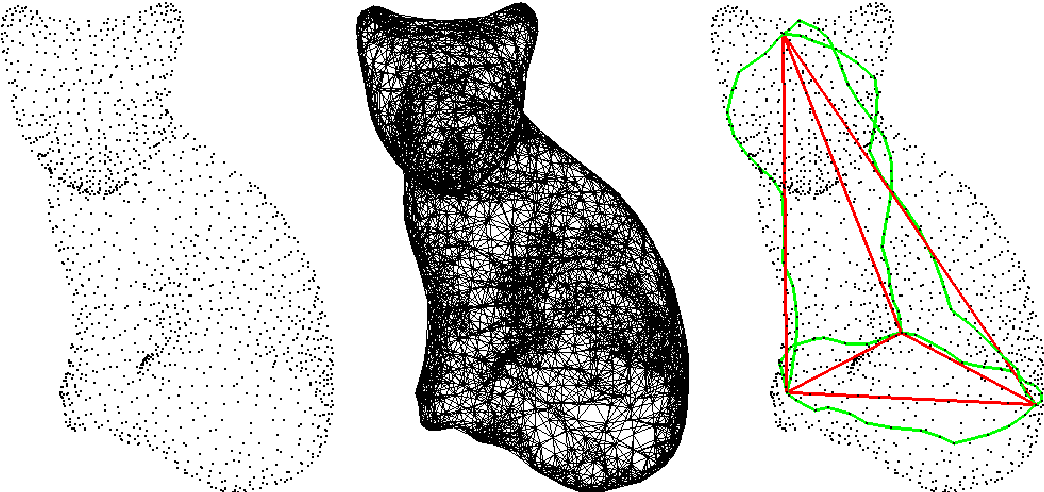
\includegraphics[width=0.5\linewidth]{triangulation}
		\caption[Triangulation of a cat]{Triangulation of a cat\footnote{Extract from \cite{hormann2002triangulating}}}
		\label{fig:triangulation}
	\end{figure}
	
	
\end{frame}
\begin{frame}
	\frametitle{Introduction}\begin{block}{constraints} 
	\begin{itemize}
\item  Approximation of objects by a finite collection of points,  
\item Take into account predefined  edges and triangulate .\end{itemize}\end{block}
	\begin{figure}[H]
		\centering
		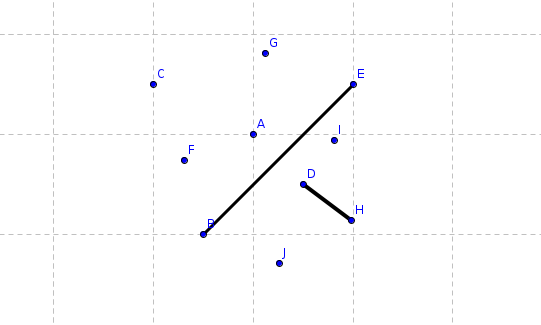
\includegraphics[width=0.4\linewidth]{graph}
		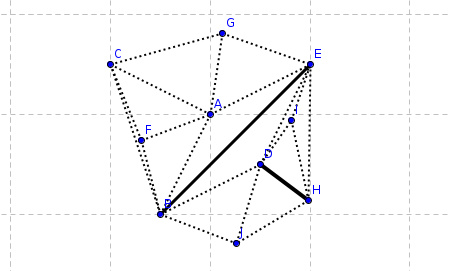
\includegraphics[width=0.4\linewidth]{graph1}
		\caption{Example of a triangulation of point set with predefined edges }
		\label{fig:polygon}
	\end{figure}
	
\end{frame}
\begin{frame}
	\frametitle{Introduction}
	\begin{block}{Questions to consider}\begin{itemize}	
	\item  Is it possible to complete a point set together with a set of initially given edges to a triangulation? 
	\item If yes, what are the techniques? \end{itemize}\end{block}This talk tries to answer these questions.
	  
\end{frame}
\begin{frame}
	\frametitle{Motivation}
	Constrained triangulations has many applications. Particularly, it is useful for\begin{itemize}\begin{block}{Applications of constrained triangulations}
	\item finite element method.\vspace{0.5cm} 
	
	\item 3D maps \vspace{0.5cm}
\item The shortest path between two points under some constraints\vspace{0.5cm}
\item Many other applications...\end{block}
\end{itemize}
\end{frame}
\begin{frame}
	\frametitle{Motivation}
%\vspace{1cm}

\begin{block}{Practice exemple}Imagine that you want to reconstruct a mountainous region and you have recorded information for a sample finitely many points in your region (eg. height).\end{block}
	%	% TODO: \usepackage{graphicx} required
		\begin{figure}[hH]\label{fig:mtfako}
			\centering
			\includegraphics[scale=.04]{Mt_Fako}
			\caption[Cameroon Mountain]{Cameroon Mountain\footnote{Extract from https://en.wikipedia.org/wiki/Mount\_Cameroon\#/media/File:Mt\_Fako.jpg}}%{https://en.wikipedia.org/wiki/Mount_Cameroon#/media/File:Mt_Fako.jpg}
	  		
		\end{figure}
\end{frame}
\begin{frame}
	You can have something like this.
	\begin{figure}[H]
		\centering
		\includegraphics[width=0.75\linewidth]{Sample}
		\caption[Sample points recorded]{sample points recorded with constrained edges\footnote{Extract from \cite{devadoss2011discrete}}}
		\label{fig:samplepoints}
	\end{figure}
	In order to make the reconstruction more realistic you would like to connect nearby points that have similar height before processing for a triangulation. Fixing some edges first and then extending them into a triangulation  is what we call constrained triangulation.
	
\end{frame}
\begin{frame}
	\frametitle{Definition}
	Let $P\subset\mathbb{R}^2$ be a finite set of points, $\mathcal{L}$ a given set of edges connecting some points of $P$.
	
	A {\color{blue}triangulation of $P$} in the plane is a subdivision of the plane by a maximal set of non-crossing edges whose vertex set is $P$.
	
	  A {\color{blue}constrained triangulation of $P$} is any triangulation of $P$ that contains every line of $\mathcal{L}$.
\end{frame}

\begin{frame}
	\frametitle{Line sweeping algorithm for constrained triangulations}
	\vspace{.3cm}
	Here we consider a set of points in the plane and some fixed edges as shown in the figure. A vertical line is sweeping from the left to the right and connecting vertices to make a triangulation.
	\begin{figure}[H]
		\centering
		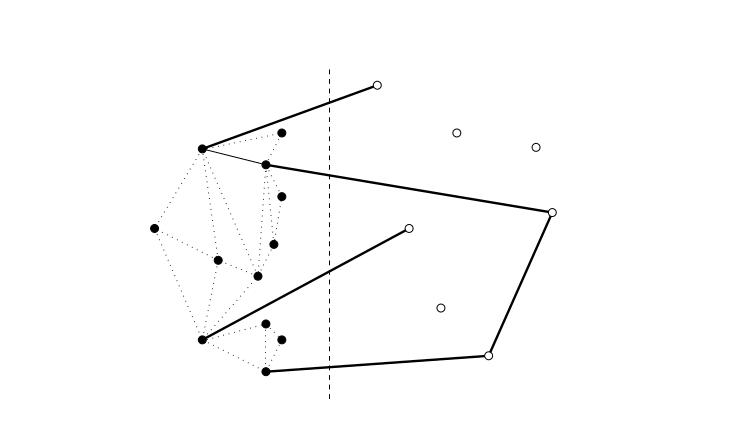
\includegraphics[scale=.25]{Line_sweeping}
		\caption[Line sweeping]{Line sweeping\footnote{Extract from \cite{edelsbrunner2001geometry}}}
		\label{fig:linesweeping}
	\end{figure}
\end{frame}
\begin{frame}
	\frametitle{Line sweeping algorithm for constrained triangulations}
\begin{block}{Algorithm}
	\begin{itemize}
		\item[$\clubsuit$] Input: a set of $n$ points in general position and a set of edges connecting some of the points. 
		\pause
		\item[$\clubsuit$] Step 1:  Sort lexicographically(i.e from the left to the right) the $n$ points and construct a triangle with the first three points.
		\pause
		\item[$\clubsuit$] Step 2: Consider the next point $p_{k+1}$ in the ordered set and connect it with all previously considered points $\left\{p_1,p_2,...,p_k\right\}$ which are visible to $p_{k+1}$.
		\pause
		\item[$\clubsuit$] Step 3: Repeat step 2 until all the points have been processed.
	\end{itemize}
\end{block}

\end{frame}

\begin{frame}
\frametitle{Line sweeping algorithm for constrained triangulations}
\vspace{.5cm}
Let $P$ a set of points and $\mathcal{L}$ a set of line segment connecting some of the points.
\begin{block}{What means to be visible ?}
	A point $A$ is visible to another point $B$ if the line segment $AB$ doesn't cross with any constrained edge.
\end{block}
\begin{block}{The algorithm terminates}
The line sweeping algorithm outputs a triangulated set of points with fixed edges.
\end{block}	\end{frame}
%\begin{figure}[H]
%	\centering
%
%	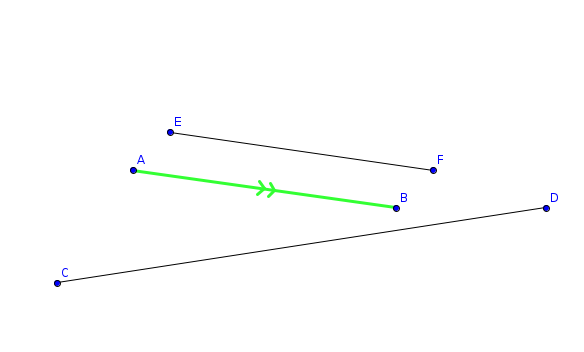
\includegraphics[scale=.09]{Visibility}
%	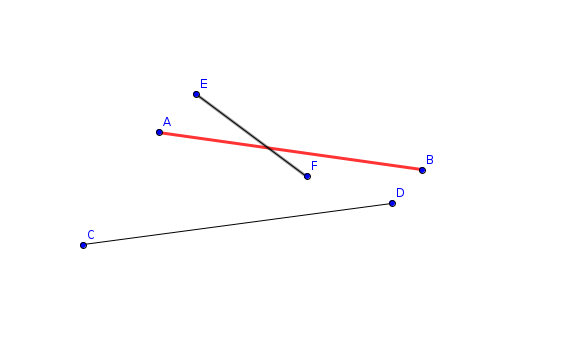
\includegraphics[scale=.09]{non-visibility}
%
%	\caption[Visibility of two points]{}
%	\label{fig:visibility}
%\end{figure}




\begin{frame}
\frametitle{Line sweeping algorithm for constrained triangulations}
\begin{figure}[H]
	%\centering
	
	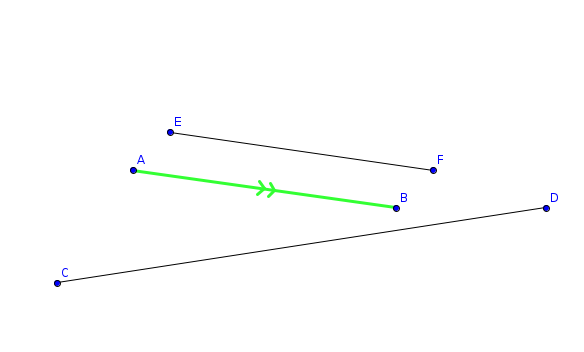
\includegraphics[scale=.25]{Visibility}
	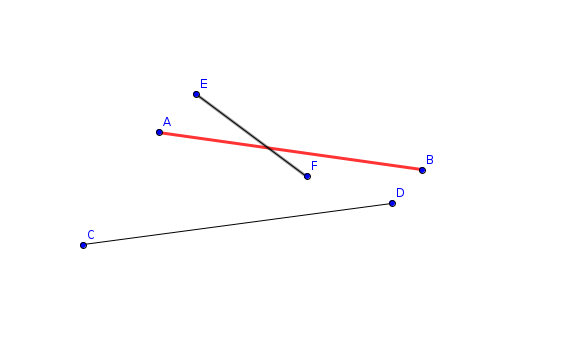
\includegraphics[scale=.25]{non-visibility}
	
	\caption{Visibility of two points}
	\label{fig:visibility}
\end{figure}
\begin{block}{Time complexity}
	The running time of this algorithm is $\mathcal{O}(n\log n)$.
\end{block}		
\end{frame}

%\begin{frame}
%\frametitle{Line sweeping algorithm for constrained triangulations}
%\vspace{.5cm}
%Let's first consider the following algorithm:
%\begin{block}
%	
%	\begin{itemize}
%		\item[$\clubsuit$] Input: Three points $A$, $B$, and $C$.
%		\item[$\clubsuit$] Output: \begin{itemize}
%			\item $0$ if the three points lie on a single line
%			\item $1$ if the triangle $ABC$ is oriented clockwise
%			\item $-1$ if the triangle $ABC$ is oriented counterclockwise
%		\end{itemize} 
%	\end{itemize}
%Call this algorithm $\textbf{\textit{Orientation}}$.	
%\end{block}	
%\end{frame}
%\begin{frame}
%	\frametitle{Line sweeping algorithm for constrained triangulations}
%	\begin{block}{Visibility}
%		Two points $A$ and $B$ are said to be visible to each other if  any  edge connecting them doesn't intersect with another line.
%	\end{block}	
%\begin{block}{Time complexity}
%	The running time of this algorithm is $\mathcal{O}(n\log n)$.
%\end{block}	
%\end{frame}
\begin{frame}
	\frametitle{Constrained Delaunay triangulations}
	Let $P$ a set of points and $\mathcal{L}$ a set of  edges connecting some of the points.
	\begin{block}{Delaunay triangulation}
  A triangulation of $P$ is a Delaunay triangulation if:
  \begin{itemize}
  	\item The circumcircle of any triangle in the triangulation does not contains any point of $P$ in its interior
  \end{itemize}
		
		
	\end{block}
\pause
\begin{block}{Constained Delaunay triangulation}
Many applications require certain type of triangulation even in the case where we have constraints edges.
\end{block}
\end{frame}
\begin{frame}
	\frametitle{Constrained Delaunay triangulations}
	Let $P$ be a set of points and $\mathcal{L}$ a set of edges which endpoints are in $P$. A triangulation $T$ is a
	constrained Delaunay triangulation (CDT) of $P$ with the edges $\mathcal{L}$ if each edge of $\mathcal{L}$ is an edge of
	$T$ and for each remaining edge $e$ of $T$ there exists a circle $\mathcal{C}$ with the following
	properties:
	\begin{itemize}
		\item The endpoints of edge $e$ are on the boundary of $\mathcal{C}$,
		\item If any vertex $v$ of $P$ is in the interior of $\mathcal{C}$ then it cannot be "seen" from at
		least one of the endpoints of $e$ (i.e., if you draw the line segments from $v$ to each endpoint of $e$ then at least one of the line segments crosses an edge of
		$\mathcal{L}$).
	\end{itemize}
\end{frame}
\begin{frame}
	\frametitle{Constrained Delaunay triangulations: an algorithm}
	\begin{block}{Algorithm(\cite{DEFLORIANI})}
		the algorithm consists of three different phase:
		\begin{itemize}
			\item Triangulation of the initial domain (a Delaunay one)
			\item Insertion of interior points
			\item Insertion of edges connecting the existing points
		\end{itemize}
		
	\end{block}
	Only the first and the last options are interesting.
\end{frame}

\begin{frame}
	%\frametitle{Constrained Delaunay triangulations}
	Let $\mathcal{L}$ be the set of constrained lines let be $l$ its cardinal.
	After insertion of a constrained line $L$, we call the set of triangles which has a crossing edge with $L$ its influence region. It's a polygon.
	\begin{figure}[H]
		\centering
		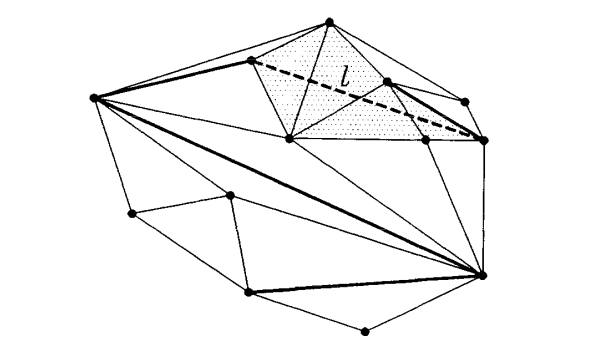
\includegraphics[width=0.7\linewidth]{zone_inf_line}
		\caption{Influence region of a line}
		\label{fig:zoneinfline}
	\end{figure}
	
\end{frame}
\begin{frame}
	\frametitle{Constrained Delaunay triangulations}
	
	\begin{block}{Insertion of lines}
		\begin{itemize}
			\item Input : Delaunay Triangulation of a set of  points.
			\item Step 1: Insert one line. It shares the influence region in two parts. Triangulate both of the part (they are polygons).
			\item Step 2: Repeat step 1 until the $l$ edges have been inserted.  
			\item Output: The CDT of the considered graph.
		\end{itemize}
	\end{block}
\begin{block}{Time complexity and correctness}
	The running time of this algorithm is $\mathcal{O}(ln\log n)$.
	
	The program output a CDT since the influence region is a polygon. 
		\end{block}
\end{frame}

\begin{frame}
	\frametitle{Conclusion}
	In summary, constrained triangulations can be determined either for given graphs, but simply for a point set on which some edges have been fixed. Different applications may require certain qualities in triangulations. I would emphasize that it depends on what you want:\begin{itemize}
		\item some algorithms just find triangulation that respects the constrained edges, 
		\item and some finds the constrained Delaunay triangulation.
	\end{itemize}  Now we know that we can find a triangulation of a given points set with constrained edges. But, now can we draw a flip graph of a constrained triangulation? (The answer is yes and further details will be presented in future work).
\end{frame}
\begin{frame}
	\frametitle{Thank you}
	\begin{center}
		\begin{LARGE}
		\textbf{\color{blue}Merci}\hfill\textbf{\color{magenta}Thank you}
			\vspace{1.7cm}
			
			
			
			
		\textbf{\color{olive}Shoukran}\hfill	\textbf{\color{cyan}Assanteni}
			\vspace{1.7cm}
			
		
			
			
			\textbf{\color{red}Medawasse}\hfill\textbf{\color{purple}\v{D}akujem}
			
			
			
		\end{LARGE}
	\end{center}
\end{frame}
\begin{frame}
	\frametitle{References}\scriptsize
	\begin{itemize}
		\item Lectures notes
		\nocite{*}
		\bibliographystyle{abbrv}
		\bibliography{References}
	\end{itemize}
\end{frame}

\end{document}